\section{Introduction to sensing}

This chapter divides into two parts, which are mostly independent from each other.
In the first part, there is a detailed description of a novel denoising filter called \gls{ac:epf}.
In environments with low ambient light conditions, any RGB camera introduces noisy pixels.
The filter removes this noise and replaces it with an averaged value of the local neighborhood.
It is shown that \gls{ac:epf} outperforms standard local denoising methods in quality while still running in real-time.
Global methods, however, show a slightly better performance, but their time performance range at about \unit[0.4]{Hz} and thus are far from real-time (and therefore not feasible in a robotic environment).
As the filter generalizes on any dimension, it can be also used on 1d sensor data, \eg readings from a gyroscope or accelerometer.

This is shown in the second part of this chapter.
Here, two ground based and one flying robot are introduced, which make use of the data filtering.
This enables the robots to use computer vision algorithms to localize themselves and share knowledge about the local environment.
A detailed analysis and comparison to start-of-the art is computed on two simulations: the here developed algorithms perform about twice as good as current state-of-the-art.
Furthermore, real-world office flights are shown.

Real-time computer vision in fast moving robots still remains a challenging task, especially when forced to use limited computing power, as it is usually the case when implemented on embedded systems. 
Different light conditions are just one aspect of this vast field of problems.
Cameras (analog as well as digital cameras) introduce noise in poor light conditions, meaning in environments with low signal-to-noise ratio.
Removing this noise usually leads to better performance of object recognition tasks in 2d and 3d images, more stable computation of features, and improve tracking results.
In~\textcite{reichabramovpapon2013} it was shown  that removal of texture from 2d images significantly improves image segmentation results.
Parts of the results shown here are also published in~\textcite{reichwoergoetterdellen2018}.

An additional application is the automatic post-production of images, which are, generally speaking, more appealing to humans; there is a big community of photographers and we deem removing noise for pure aesthetic value as also important.
One application of the here presented filter is shown in \figref{fig:sensor_introduction_lena}.

Still, the filter generalizes well on arbitrary dimensions.
In a second part it is shown how to apply the same mechanisms to an arbitrary number of dimensions, enabling the filter to run on any physical measurement, for example on 1d sensor data obtained from an accelerometer, gyroscope, or \gls{ac:gps} tracker.

\begin{figure}
    \centering
    \begin{subfigure}[]{0.475\textwidth}
        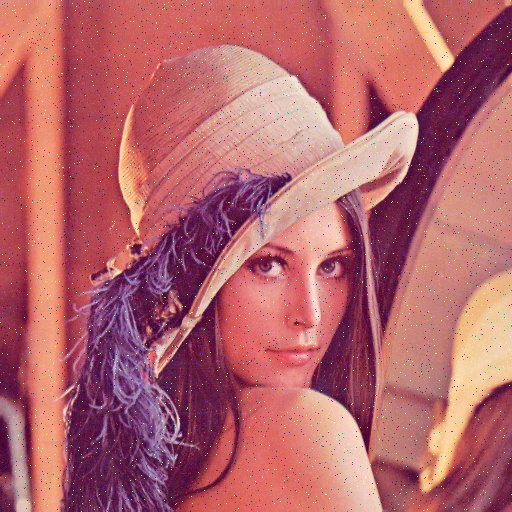
\includegraphics[width=\textwidth]{./figures/sensor/introduction_lena_noisy.jpg}
        \caption{Noisy test image.}
        \label{fig:sensor_introduction_lena_noisy}
    \end{subfigure}\hfill%
    \begin{subfigure}[]{0.475\textwidth}
        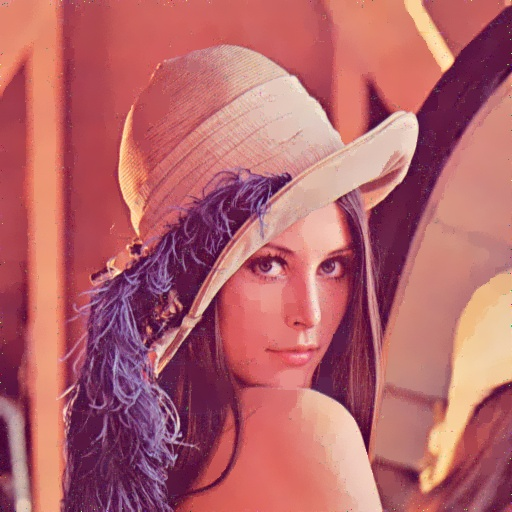
\includegraphics[width=\textwidth]{./figures/sensor/introduction_lena_edgefilter.jpg}
        \caption{Denoised test image.}
        \label{fig:sensor_introduction_lena_denoised}
	\end{subfigure}
  \caption{Even today, denoising remains a challenging task. The here proposed real-time denoising filter is called \gls{ac:epf}.}
  \label{fig:sensor_introduction_lena}
\end{figure}

Removing noise is a two-step process: First a noisy pixel needs to be identified as such, second it needs to be smoothed out. 
Both steps offer a wide range of problems.
In the first step a noisy pixel needs to be defined in a mathematical sense.
This means that a similarity criterion must be found.
However, similarities can exist on different scales, \ie between adjacent pixels or groups of pixels, as it is the case for texture.
In the second step a target value needs to be computed, which replaces the noisy pixel.
This target value should, again, only depend on the local neighborhood.

Removing noise has a long history in science. 
Most notable is the Gaussian Filter. 
It works by convoluting an image with a Gaussian function and thus works as a simple low-pass filter, attenuating high frequency signals~\cite[p. 257f]{gonzalezwoods2002}. 
As edges are also a high-frequency signal, they will be blurred out, too.

Noise in images is usually distinguished using a threshold. 
This thresholds can be either learned using a training set of images, as in support vector machines~\cite{yang2010svm} and \gls{ac:ann}~\cite{muneyasu1995realization,pandey2016anatomization}, or the threshold may be computed from the surrounding pixel values, as in~\cite{du2011dynamic}. 
\cite{lev1977iterative} identified similar pixels by detecting edges and iteratively replacing the intensity of the pixel by the mean of all pixels in a small environment.

Another approach is presented in~\cite{tomasi1998bilateral}: The so called bilateral filter blurs neighboring pixels depending on their combined color and spatial distance. 
Hence, texture and noise, which has small deviation from the mean can be blurred without affecting boundaries. 
This leads to a trade-off: large blurring factors are needed to smooth out high level of noise, having the consequence that edges are not preserved anymore.

Another wide class of algorithms denoise by averaging. 
This averaging may happen locally as in the Gaussian smoothing model~\cite{lindenbaum1994gabor}, the anisotropic smoothing model~\cite{perona1990scale,alvarez1992image}, based on neighborhood filtering as in the already mentioned bilateral filter~\cite{tomasi1998bilateral}, using local variations as in~\cite{rudin1992nonlinear}, or based on the wavelet thresholding method~\cite{donoho1995noising}.

All this powerful methods have one common drawback: they all smooth small scaled noise and preserve color edges, however are not able to distinguish between a color edge and large scaled noise, \eg outliers. 
Outliers are a common problem in any sensor based application, as in accelerometers or gyroscopes, but also in 2d-RGB cameras, where high ISO settings often pose a big problem. 
More recent methods, which achieve this goal~\cite{dabov2007image,zoran2011learning,mairal2009non}, do not perform in real-time.
The here presented approach has the following features:

\begin{enumerate}
  \item smooths out small scaled noise,
  \item smooths out outliers,
  \item still preserves color edges, and
  \item performs in real-time.
\end{enumerate}

In the following section, a mathematical formulation of the filter in the discrete and continuous domain is introduced. 
Afterwards, results are shown and compared to current state-of-the-art using two image data sets.
Then, the generalization to arbitrary dimensions is described and experiments on artificial data shown.
This will be followed by a detailed discussion and conclusion.
